\newcommand{\Up}{\ket{\Uparrow}}
\newcommand{\Right}{\ket{\Rightarrow}}
\newcommand{\LUp}{\bra{\Uparrow}}
\newcommand{\LRight}{\bra{\Rightarrow}}
In the following, we will examine a 1D Ising Hamiltonian of the form 
\begin{equation}
    H=-J\sum_{n=1}^L\sigmax{}_{,n}\sigmax{}_{,n+1}-g\sum_{n=1}^L\sigmaz{}_{,n}-h\sum_{n=1}^L\sigmax{}_{,n}
\end{equation}
with $L$ describing the number of lattice sites.

\section{Single-Site Expectation Values}
Initializing our 1-dimensional Ising chain to the all spin-up state (i.e. $\ket{\uparrow\uparrow...\uparrow}\equiv\Up$), we obtain the expected expectation values
\begin{align}
    \LUp\sigmax{}_{,i}\Up &= 0 \\
    \LUp\sigmaz{}_{,i}\Up &= 1
\end{align}
for every $i$, where $i$ is the site on which the operator acts. On the other hand, initializing the state $\ket{\rightarrow\rightarrow...\rightarrow}\equiv\Right$, with $\ket{\rightarrow}=\frac{1}{\sqrt{2}}(\ket{\uparrow}+\ket{\downarrow})$, we obtain
\begin{align}
    \LRight\sigmax{}_{,i}\Right &= 1 \\
    \LRight\sigmaz{}_{,i}\Right &= 0
\end{align}
The numerical calculations match these values.


\section{Energy of 1D Ising Chain}
The expectation values of the energy for the states $\Up$ and $\Right$ for different values of $g$ are depicted in Fig. \ref{fig:energy-g}. We see that the energy decreases linearly with increasing $g$ for the $\Up$ state, but stays constant for the $\Right$ state. Mathematically, this is the case, because $g$ is a linear coefficient in front of the single site $\sigmaz{}_{,i}$-operator. According to the previous section, every site adds $-g$ if the state is $\Up$, but does not contribute to the energy if the state is $\Right$.\\
Physically, the parameter $g$ corresponds to an applied magnetic field in the $z$-direction. The anti-alignment of the spins with the magnetic field is energetically favorable. The individual $\ket{\rightarrow}$ states, however, are neither aligned, nor anti-aligned with the field and experience therefore no energy shift. The fact that the $\Right$-state has a lower energy for $g=\num{0.5}$ comes from the fact that $\sigmax{}$ alignment of nearest neighbors is energetically favorable.  
\begin{figure}[htbp]
    \centering
    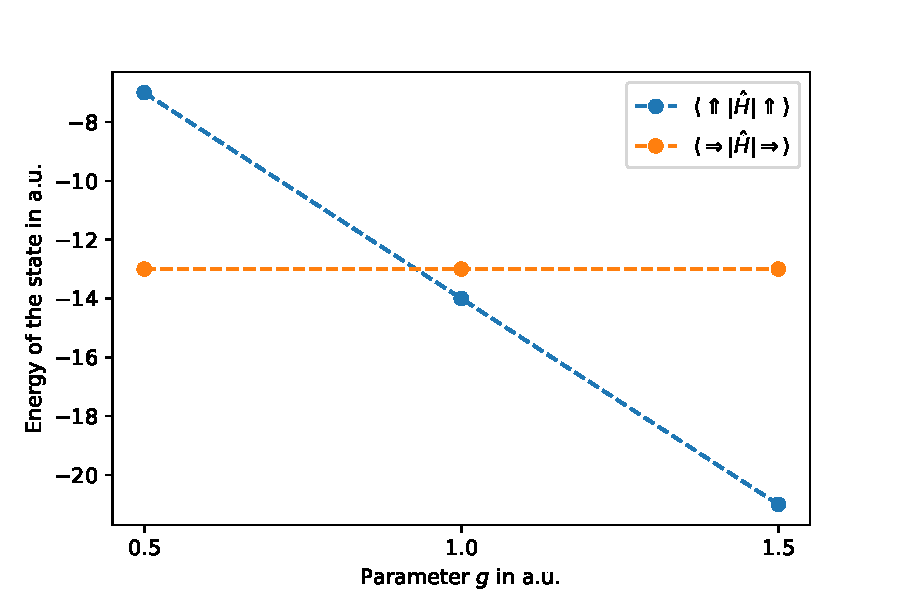
\includegraphics[width=0.7\textwidth]{energy-g.pdf}
    \caption{Expectation value of the states $\Up$ and $\Right$ for a chain length of $L=\num{14}$, $J=1$ and different values of $g$.}
    \label{fig:energy-g}
\end{figure}
\FloatBarrier
\section{Equal-Time Correlations and Magnetization}

The equal time correlations $\langle \sigmax{}_{,L/4}\sigmax{}_{,j}\rangle $ for the ground state of the Ising Hamiltonian with $L=30$, $J=1$ and different values for $g$ can be seen in Fig. \ref{fig:correlation-g}. For $g\ll 1$, the correlation is roughly constant and approaches 1. For larger values of $g$ we find a linear decrease of the correlations in the logarithmic scaled plot, suggesting an exponential decrease of the correlation. In effect, the magnetic field causes the spins to flip on average, causing a smaller correlation. The downturn for the final values of $j$ is due to the open boundary conditions. Those boundary conditions are also the reason why $L/4$ is used as the reference site.\\
Using this data, we can extract the magnetization for different values of $g$. For the magnetization, the following realtion holds:
\begin{equation}
    \langle \sigmax{}_{,i}\sigmax{}_{,j}\rangle \rightarrow m^2\,\text{for}\, |i-j|\rightarrow \infty
\end{equation}
This means that the correlations approach the magnetization squared for large distances. In our model, we use $i=L/4$ and $j=3L/4$  as an approximation of the magnetization, to exclude the aforementioned boundary effects. The plot can be seen in Fig. \ref{fig:magnetization}. We can see a phase transition occuring at $g=1$. %Since the magnetization is low for large magnetic fields, we can conclude that this Ising chain behaves \todo[]{ferromagnetic then anitferromagnetic? Does this make sense?}
\begin{figure}[htbp]
    \centering
    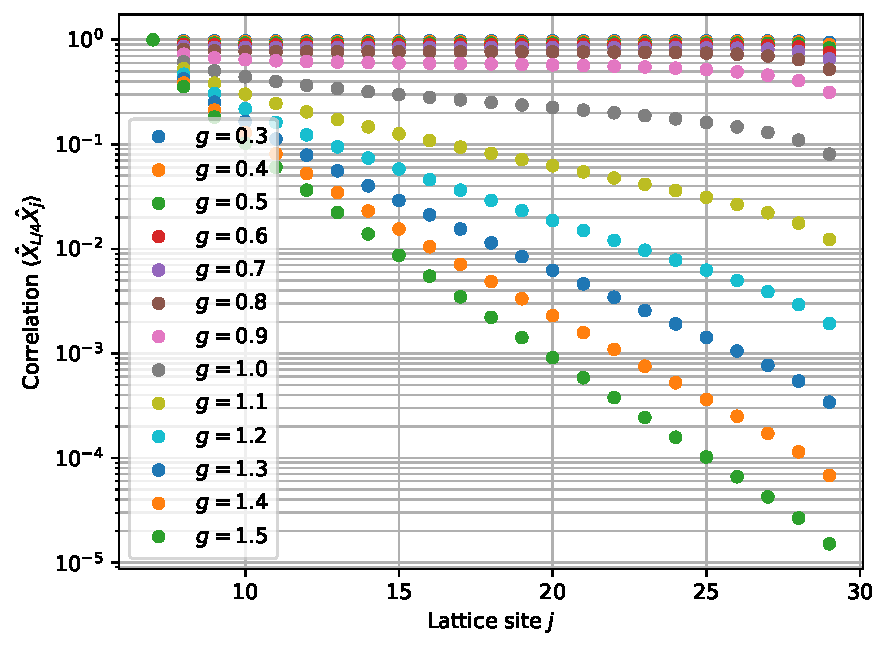
\includegraphics[width=0.7\textwidth]{T4.2_d_all.pdf}
    \caption{Correlations $\langle \sigmax{}_{,L/4}\sigmax{}_{,j}\rangle $ of the ground state of the Ising Hamiltonian against the lattice site $j$ for different values of $g$ on a logarithmic scale. We can see that for $g>1$, the plots approach a linear function on the logarithmic scale.}
    \label{fig:correlation-g}
\end{figure}
\begin{figure}[htbp]
    \centering
    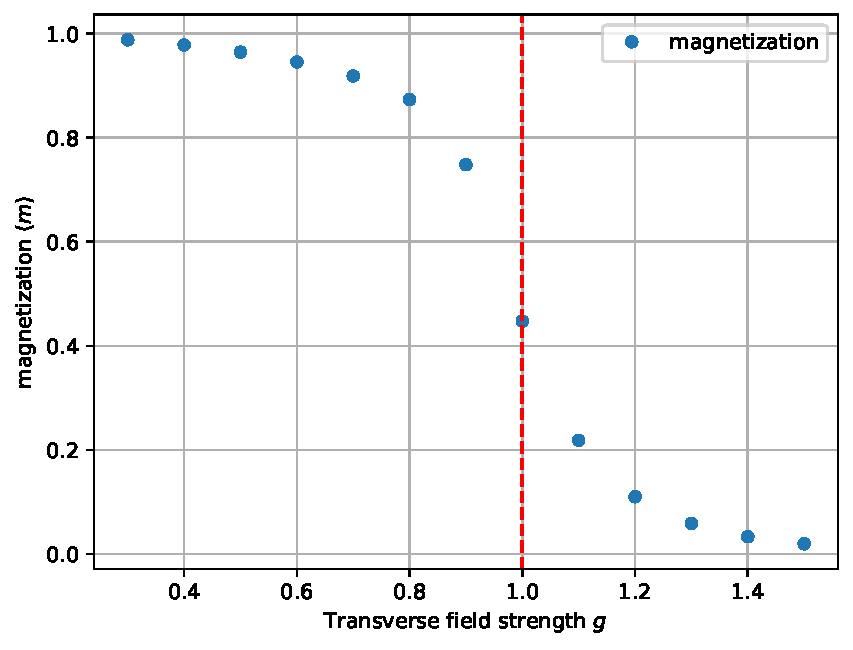
\includegraphics[width=0.7\textwidth]{T4.2_c.pdf}
    \caption{Magnetization of the system with respect to $g$. We can see a phase transition at $g=1$.}
    \label{fig:magnetization}
\end{figure}

\section{Connected Correlations and Correlation Length}
The connected correlations are defined as 
\begin{equation}
    C(j) = \langle \sigmax{}_{,L/4}\sigmax{}_{,j}\rangle - \langle \sigmax{}_{,L/4}\rangle\langle\sigmax{}_{,j}\rangle
\end{equation}
This data can be seen  in Fig. \ref{fig:connected-corr}
\begin{figure}[htbp]
    \centering
    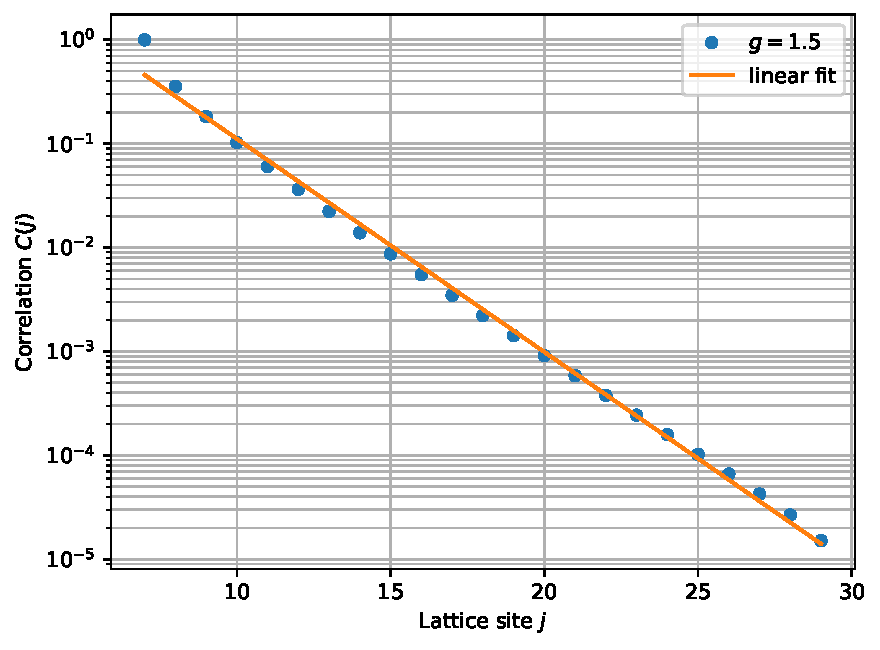
\includegraphics[width=0.7\textwidth]{T4.2_d_fit.pdf}
    \caption{Linear fit in the logarithmic plot of the correlations. This can be used to extract the correlation length $\xi$.}
    \label{fig:connected-corr}
\end{figure}
Since the curve is linear in the logarithmic plot, we obtain data of the kind
\begin{equation}
    C(j) \propto \exp\left(-\frac{|j-L/4|}{\xi}\right)
\end{equation}
We now use a linear fit of the logarithmic data
\begin{align}
    x = j & &y = \log\left(C(j)\right)
\end{align}
Therefore, we obtain 2 parameters $a, b$, that describe our fit-function
\begin{align}
    f(x) = a + b x = y
\end{align}
or according to our logarithmic fit:
\begin{align}
    C(j) = e^a \, \exp\left(b j\right)
\end{align}
Therefore, we can directly extract the correlation length $\xi$ as
\begin{equation}
    \xi = -1/b
\end{equation}


Now, we want to take a look at the dependence of the correlation length on the strength of the external magnetic field, which strength is given by $g$.
We therefore simulated a lot of additional ground states for different $g$ values and extracted the correlation length through the linear fit, as shown exemplary in the section above.
The obtained data is shown in \autoref{fig:corr_length_vs_g}.
One can clearly see that the correlation length converges to 0 for $g\rightarrow\infty$.
This is in accordance to our expectation.
In the case of a very large external fields, all spins are going to follow its direction.
We therefore end up with a fully separable state, that has no correlation between the sites.%\todo[]{is this true? a fully seperable state can indeed have high correlations, right? Wouldnt no correlation mean disorder, i.e. you cannot predict which state is at j knowing the state of i?}
\begin{equation}
    \ket{\Psi}_{\text{GS, } g\rightarrow\infty} = \ket{\uparrow} \otimes \ket{\uparrow} \otimes \dots \otimes \ket{\uparrow}
\end{equation}
This limit can also be seen in the plot.

Furthermore, we expect the correlation length to diverge at the critical point $g=1$.
This is not quite the case in our simulation.
If we were to show the additional data for $g<1$ it would look like an exponential decay starting at $g=0$.
This is due to the fact, that the divergence only happens in the thermodynamic limit, but we are only considering finite systems.
Still, we can clearly see a large increase in the correlation length at the critical point $g=1$.
\begin{figure}[htbp]
    \centering
    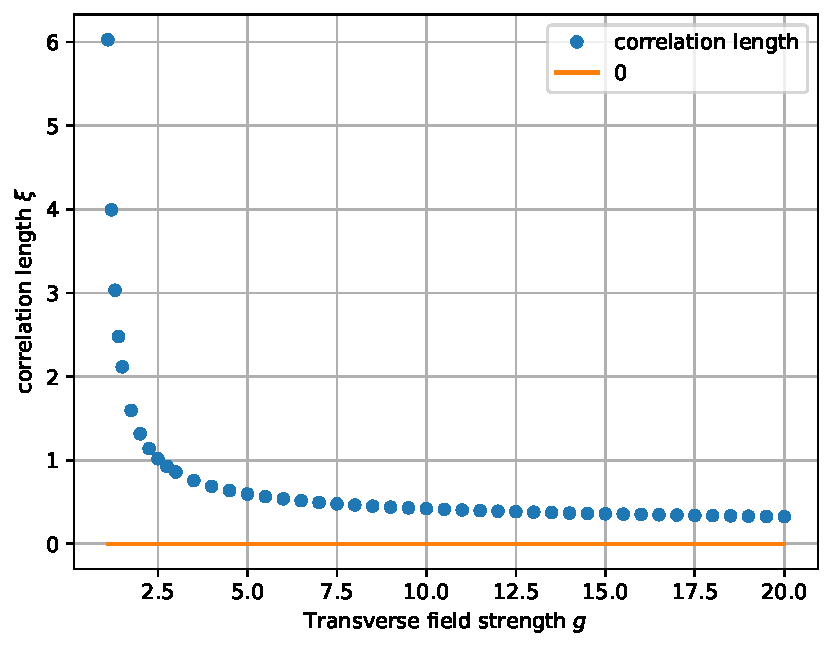
\includegraphics[width=0.7\textwidth]{T4.2_d_xi_vs_g.pdf}
    \label{fig:corr_length_vs_g}
    \caption{Visualization of the correlation length $\xi$ with respect to $g$. One can see the steady decrease to $\xi\rightarrow0$ for $g\rightarrow\infty$.}
\end{figure}

